\documentclass[border=5pt]{standalone}
\usepackage{tikz}
\usetikzlibrary{calc}
\usepackage{amsmath}
\begin{document}
    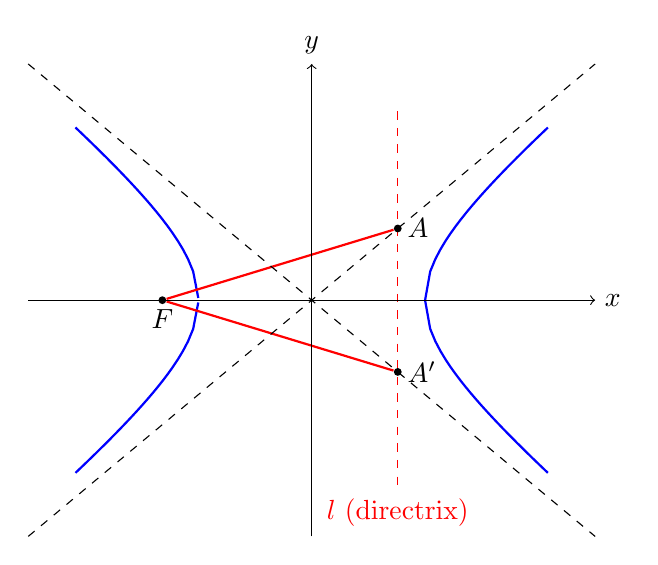
\begin{tikzpicture}[scale=1.2]
        % Draw hyperbola
        \draw[blue, thick, domain=1.2:2.5] plot (\x, {sqrt((\x*\x/1.44) - 1)});
        \draw[blue, thick, domain=1.2:2.5] plot (\x, {-sqrt((\x*\x/1.44) - 1)});
        \draw[blue, thick, domain=-2.5:-1.2] plot (\x, {sqrt((\x*\x/1.44) - 1)});
        \draw[blue, thick, domain=-2.5:-1.2] plot (\x, {-sqrt((\x*\x/1.44) - 1)});

        % Draw directrix
        \draw[dashed, red] (0.911,2) -- (0.911,-2) node[below] {$l$ (directrix)};

        % Draw focus
        \node[circle, fill, inner sep=1pt] (F) at (-1.5804,0) {};
        \node[below] at (F) {$F$};

        % Draw points A and A'
        \node[circle, fill, inner sep=1pt] (A) at (0.911,0.759) {};
        \node[circle, fill, inner sep=1pt] (A') at (0.911,-0.759) {};
        \node[right] at (A) {$A$};
        \node[right] at (A') {$A'$};

        % Draw triangle
        \draw[red, thick] (A) -- (F) -- (A') -- cycle;

        % Draw asymptotes
        \draw[dashed] (-3,-2.5) -- (3,2.5);
        \draw[dashed] (-3,2.5) -- (3,-2.5);

        % Draw axes
        \draw[->] (-3,0) -- (3,0) node[right] {$x$};
        \draw[->] (0,-2.5) -- (0,2.5) node[above] {$y$};
    \end{tikzpicture}
\end{document}
